\documentclass [12pt] {article}
\usepackage[]{graphicx}\usepackage[]{color}


%% maxwidth is the original width if it is less than linewidth
%% otherwise use linewidth (to make sure the graphics do not exceed the margin)
\makeatletter
\def\maxwidth{ %
  \ifdim\Gin@nat@width>\linewidth
    \linewidth
  \else
    \Gin@nat@width
  \fi
}
\makeatother

\definecolor{fgcolor}{rgb}{0.345, 0.345, 0.345}
\newcommand{\hlnum}[1]{\textcolor[rgb]{0.686,0.059,0.569}{#1}}%
\newcommand{\hlstr}[1]{\textcolor[rgb]{0.192,0.494,0.8}{#1}}%
\newcommand{\hlcom}[1]{\textcolor[rgb]{0.678,0.584,0.686}{\textit{#1}}}%
\newcommand{\hlopt}[1]{\textcolor[rgb]{0,0,0}{#1}}%
\newcommand{\hlstd}[1]{\textcolor[rgb]{0.345,0.345,0.345}{#1}}%
\newcommand{\hlkwa}[1]{\textcolor[rgb]{0.161,0.373,0.58}{\textbf{#1}}}%
\newcommand{\hlkwb}[1]{\textcolor[rgb]{0.69,0.353,0.396}{#1}}%
\newcommand{\hlkwc}[1]{\textcolor[rgb]{0.333,0.667,0.333}{#1}}%
\newcommand{\hlkwd}[1]{\textcolor[rgb]{0.737,0.353,0.396}{\textbf{#1}}}%

\usepackage{framed}
\makeatletter
%\newenvironment{kframe}{%
% \def\at@end@of@kframe{}%
% \ifinner\ifhmode%
%  \def\at@end@of@kframe{\end{minipage}}%
%  \begin{minipage}{\columnwidth}%
% \fi\fi%
% \def\FrameCommand##1{\hskip\@totalleftmargin \hskip-\fboxsep
% \colorbox{shadecolor}{##1}\hskip-\fboxsep
     % There is no \\@totalrightmargin, so:
%     \hskip-\linewidth \hskip-\@totalleftmargin \hskip\columnwidth}%
% \MakeFramed {\advance\hsize-\width
%   \@totalleftmargin\z@ \linewidth\hsize
%   \@setminipage}}%
% {\par\unskip\endMakeFramed%
% \at@end@of@kframe}
%\makeatother
%\definecolor{shadecolor}{rgb}{.97, .97, .97}
%\definecolor{messagecolor}{rgb}{0, 0, 0}
%\definecolor{warningcolor}{rgb}{1, 0, 1}
%\definecolor{errorcolor}{rgb}{1, 0, 0}
%\newenvironment{knitrout}{}{} % an empty environment to be redefined in TeX
\usepackage{csquotes}
\usepackage{alltt}
\usepackage{standalone}
\usepackage{amsfonts,amsmath, amssymb,bm}
\usepackage{graphicx,subfigure} %,float}
%\usepackage[export]{adjustbox}
\usepackage{setspace}
\usepackage{lipsum}
\usepackage[utf8]{inputenc} %french 
\usepackage{floatrow}
\usepackage{verbatimbox} %obtain-verbatim-text-in-a-footnote
\floatsetup[table]{capposition=top}
\floatsetup[figure]{capposition=top}
\usepackage{longtable}
\usepackage{indentfirst}
\usepackage[labelfont=bf, labelsep=period]{caption} %a dot instead of colon in table/figure captions
%\usepackage[labelfont=bf,labelsep=space]{caption}
\usepackage[font=bf]{caption} %bold all captions
\usepackage{titlesec} %add dot after \section number
\titlelabel{\thetitle.\enskip} %add dot after \section number \enskip, \quad, \qquad leave a horizontal space of respectively half an em, one em and two ems
\usepackage[top=1in, bottom=1in, left=1in, right=1in] {geometry}
\usepackage[colorlinks=true, linkcolor=blue, anchorcolor = blue, urlcolor  = blue, citecolor = blue]{hyperref}
\usepackage{dcolumn}
\usepackage[sort,comma,semicolon]{natbib}
\bibpunct{(}{)}{;}{a}{}{,}
\usepackage{framed} %for framed box%
%\setlength{\bibsep}{0.0pt}
%\usepackage[nolists,noheads]{endfloat}
\newcolumntype{d} [1]{D{.}{.}{#1}}
\usepackage{fancyhdr} %loads the package
\usepackage{fancyvrb}
\pagestyle{fancy} %tells the Latex you are going to make changes to the header/footer
\fancyhf{} %clears previous formatting
\rfoot{\thepage} %put the page number on the right side of the footer
\renewcommand{\headrulewidth}{0pt}
\setcounter{page} {0}
%\usepackage[none]{hyphenat} 
\usepackage{appendix}
\usepackage[section]{placeins}
%Latex tree package
\usepackage{lscape}
\usepackage{listings} %%use for R, Java code

\lstset{frame=tb,
  language=R,
  aboveskip=3mm,
  belowskip=3mm,
  showstringspaces=false,
  columns=flexible,
  basicstyle={\small\ttfamily},
  numbers=none,
  numberstyle=\tiny\color{gray},
  keywordstyle=\color{blue},
  commentstyle=\color{dkgreen},
  stringstyle=\color{mauve},
  breaklines=false,
  breakatwhitespace=true,
  tabsize=3
}

\usepackage{tikz}
\usepackage{verbatim}
\usepackage{hanging}
\usetikzlibrary{shapes}
\usepackage{ragged2e}
\usetikzlibrary{arrows,positioning}
\usepackage{xspace}

\renewcommand{\footnotesize}{\small} % 10pt footnotes in 11pt doc instead of 9pt

\usepackage[hang, flushmargin,splitrule,multiple]{footmisc}
\usepackage{etoolbox}

\makeatletter%%
\patchcmd{\@makefntext}{%
\ifFN@hangfoot
\bgroup}%
{%
\ifFN@hangfoot
\bgroup\def\@makefnmark{\rlap{\normalfont\@thefnmark.}}}{}{}%
% %%%
\patchcmd{\@makefntext}{%
\ifdim\footnotemargin>\z@
\hb@xt@ \footnotemargin{\hss\@makefnmark}}%
{%
\ifdim\footnotemargin>\z@
\hb@xt@ \footnotemargin{\@makefnmark\hss}}{}{}%
\makeatother

\setlength{\footnotemargin}{1.25em} % Between marker and text
\setlength{\skip\footins}{1\baselineskip} % Between main text and note rule
%\setlength{\footnotesep}{\skip\footins} % Between footnotes [= previous]

%\renewcommand{\hangfootparskip}{0pt}
%\renewcommand{\hangfootparindent}{1em}

\newcommand{\A}{\ensuremath{\mathcal{A}}\xspace}
\newcommand{\B}{\ensuremath{\mathcal{B}}\xspace}
\newcommand\pa[1]{\ensuremath{\left(#1\right)}}
%\graphicspath{{images/}} %path for inputting graphics

\begin {document}
\renewcommand{\thefootnote}{\fnsymbol{footnote}}
\title{ \Large{How does economic performance affect political instability\vspace*{.2in}}}
\author{ Chong Chen\footnotemark[1]}
\date{\today}
%\date{}
\footnotetext[1] {PhD Student, Department of Political Science, Duke University. Email: \href{mailto:chong.chen@duke.edu}{chong.chen@duke.edu}.}


\maketitle
\thispagestyle{empty}
\singlespacing
\renewcommand{\thefootnote}{\arabic{footnote}}

\renewcommand{\abstractname}{\large Abstract}
\begin{abstract}
  \bigskip
	\noindent
How do periods of conflict and peace shape gender hierarchy around the world? 
\end{abstract}



\newpage
\setlength{\parskip}{-2em}
%\setlength{\parindent}{1cm}
\doublespacing
\setcounter{page} {1}

	
\section{Introduction}
\label{intro}
\vspace*{.2in}

This is a test paper!

\section{Results}
\label{result}
\vspace*{.2in}


%EDA

\begin{figure}
\centering
\caption{EDA}
\label{eda}
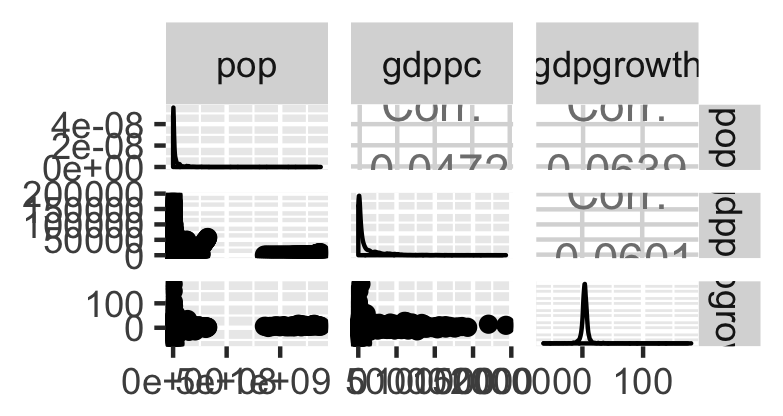
\includegraphics[scale =.5]{images/eda.png}
\end{figure}



%fig1
\begin{figure}
\centering
\caption{Coefficient Plot for Model 1 and Model 5}
\label{cof1}
\subfigure[model 1]{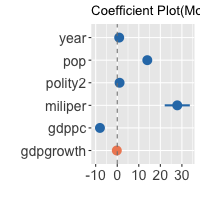
\includegraphics[scale =1]{images/coefm1_lm.png}}
\subfigure[model 5]{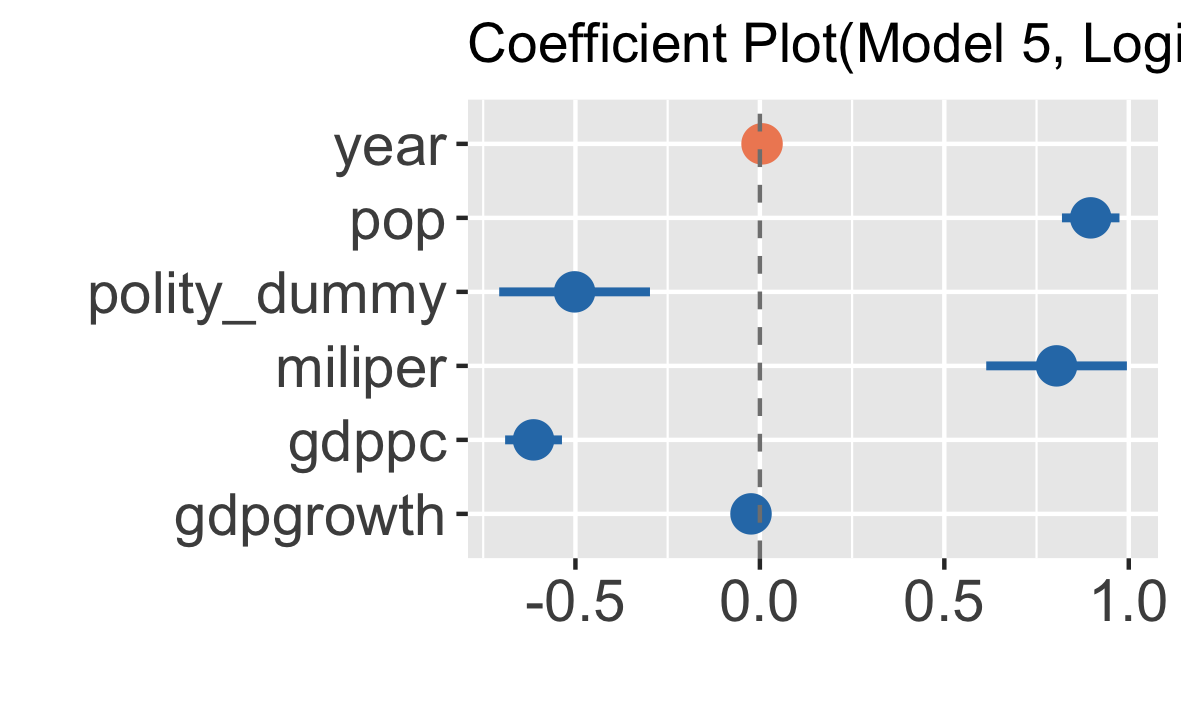
\includegraphics[scale =.2]{images/coefm1_m2}}
\end{figure}


% density plot

\begin{figure}
\centering
\caption{Density Plot for Model 5}
\label{cof2}
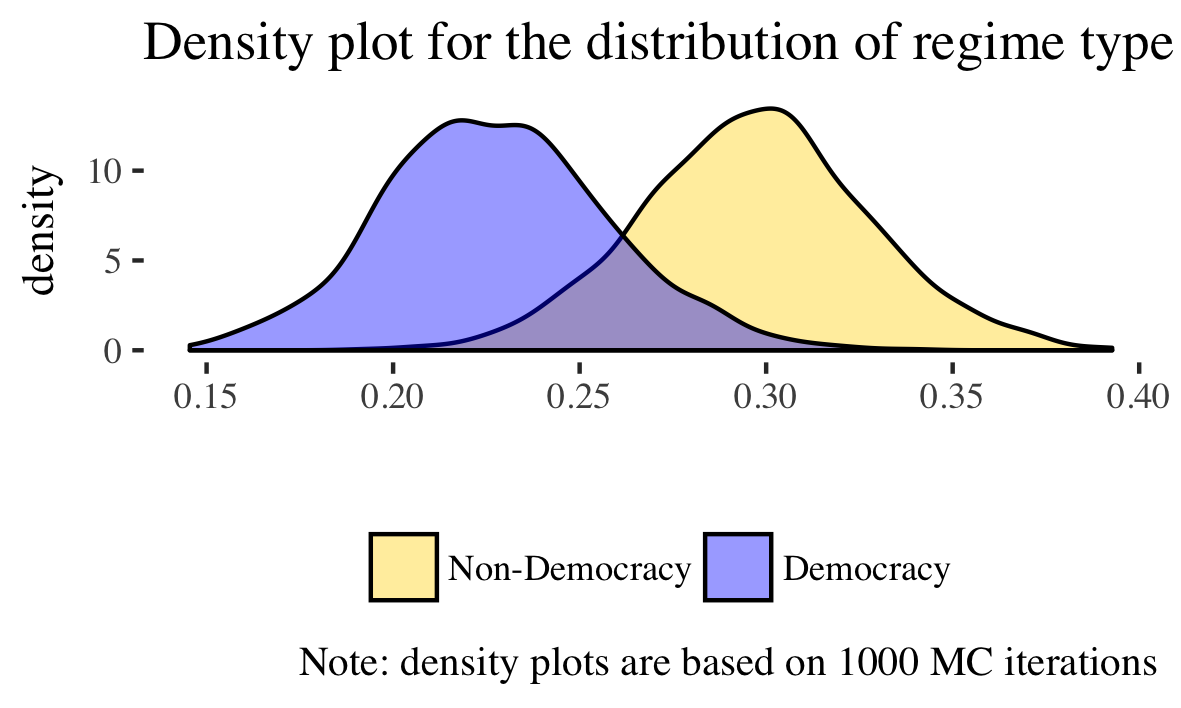
\includegraphics[scale =.5]{images/m2_density.png}
\end{figure}



\begin{table}
\begin{center}
\begin{tabular}{l c c c c c }
\hline
 & Model 1 & Model 2 & Model 3 & Model 4 & Model 5 \\
\hline
(Intercept)                  & $-1988.52^{***}$ & $-36.99$      & $0.00$   & $-27.66^{*}$  & $-23.25$      \\
                             & $(374.78)$       & $(19.16)$     & $(0.00)$ & $(12.98)$     & $(13.06)$     \\
Polity IV score              & $1.09^{***}$     & $-0.01$       & $0.00$   & $-0.01$       &               \\
                             & $(0.23)$         & $(0.01)$      & $(0.00)$ & $(0.01)$      &               \\
Population(log)              & $13.95^{***}$    & $1.45^{***}$  & $0.00$   & $0.89^{***}$  & $0.90^{***}$  \\
                             & $(0.87)$         & $(0.05)$      & $(0.00)$ & $(0.04)$      & $(0.04)$      \\
GDP per captia (log)         & $-8.02^{***}$    & $-0.89^{***}$ & $0.00$   & $-0.67^{***}$ & $-0.61^{***}$ \\
                             & $(0.94)$         & $(0.05)$      & $(0.00)$ & $(0.04)$      & $(0.04)$      \\
GDP growth (\%)              & $-0.20$          & $-0.07^{***}$ & $0.00$   & $-0.02^{**}$  & $-0.02^{**}$  \\
                             & $(0.21)$         & $(0.01)$      & $(0.00)$ & $(0.01)$      & $(0.01)$      \\
\% of Armed forces personnel & $27.85^{***}$    & $2.95^{***}$  & $0.00$   & $0.88^{***}$  & $0.80^{***}$  \\
                             & $(2.97)$         & $(0.15)$      & $(0.00)$ & $(0.10)$      & $(0.10)$      \\
year                         & $0.91^{***}$     & $0.01$        & $0.00$   & $0.01$        & $0.01$        \\
                             & $(0.19)$         & $(0.01)$      & $(0.00)$ & $(0.01)$      & $(0.01)$      \\
Polity(dummy)                &                  &               &          &               & $-0.50^{***}$ \\
                             &                  &               &          &               & $(0.10)$      \\
\hline
R$^2$                        & 0.09             &               &          &               &               \\
Adj. R$^2$                   & 0.09             &               &          &               &               \\
Num. obs.                    & 3687             & 3687          & 3687     & 3687          & 3687          \\
RMSE                         & 79.52            &               & 0.00     &               &               \\
AIC                          &                  & 10996.85      &          & 3083.83       & 3062.53       \\
BIC                          &                  & 11046.55      &          & 3127.32       & 3106.02       \\
Log Likelihood               &                  & -5490.42      &          & -1534.92      & -1524.27      \\
Deviance                     &                  & 1655.01       &          & 3069.83       & 3048.53       \\
\hline
\multicolumn{6}{l}{\scriptsize{$^{***}p<0.001$, $^{**}p<0.01$, $^*p<0.05$}}
\end{tabular}
\caption{Regression Results}
\label{table:coefficients}
\end{center}
\end{table}




\end{document}
	
